\thispagestyle{fancy}

\begin{appendices}

\chapter{Tables}

    \begin{figure}
        \centering
        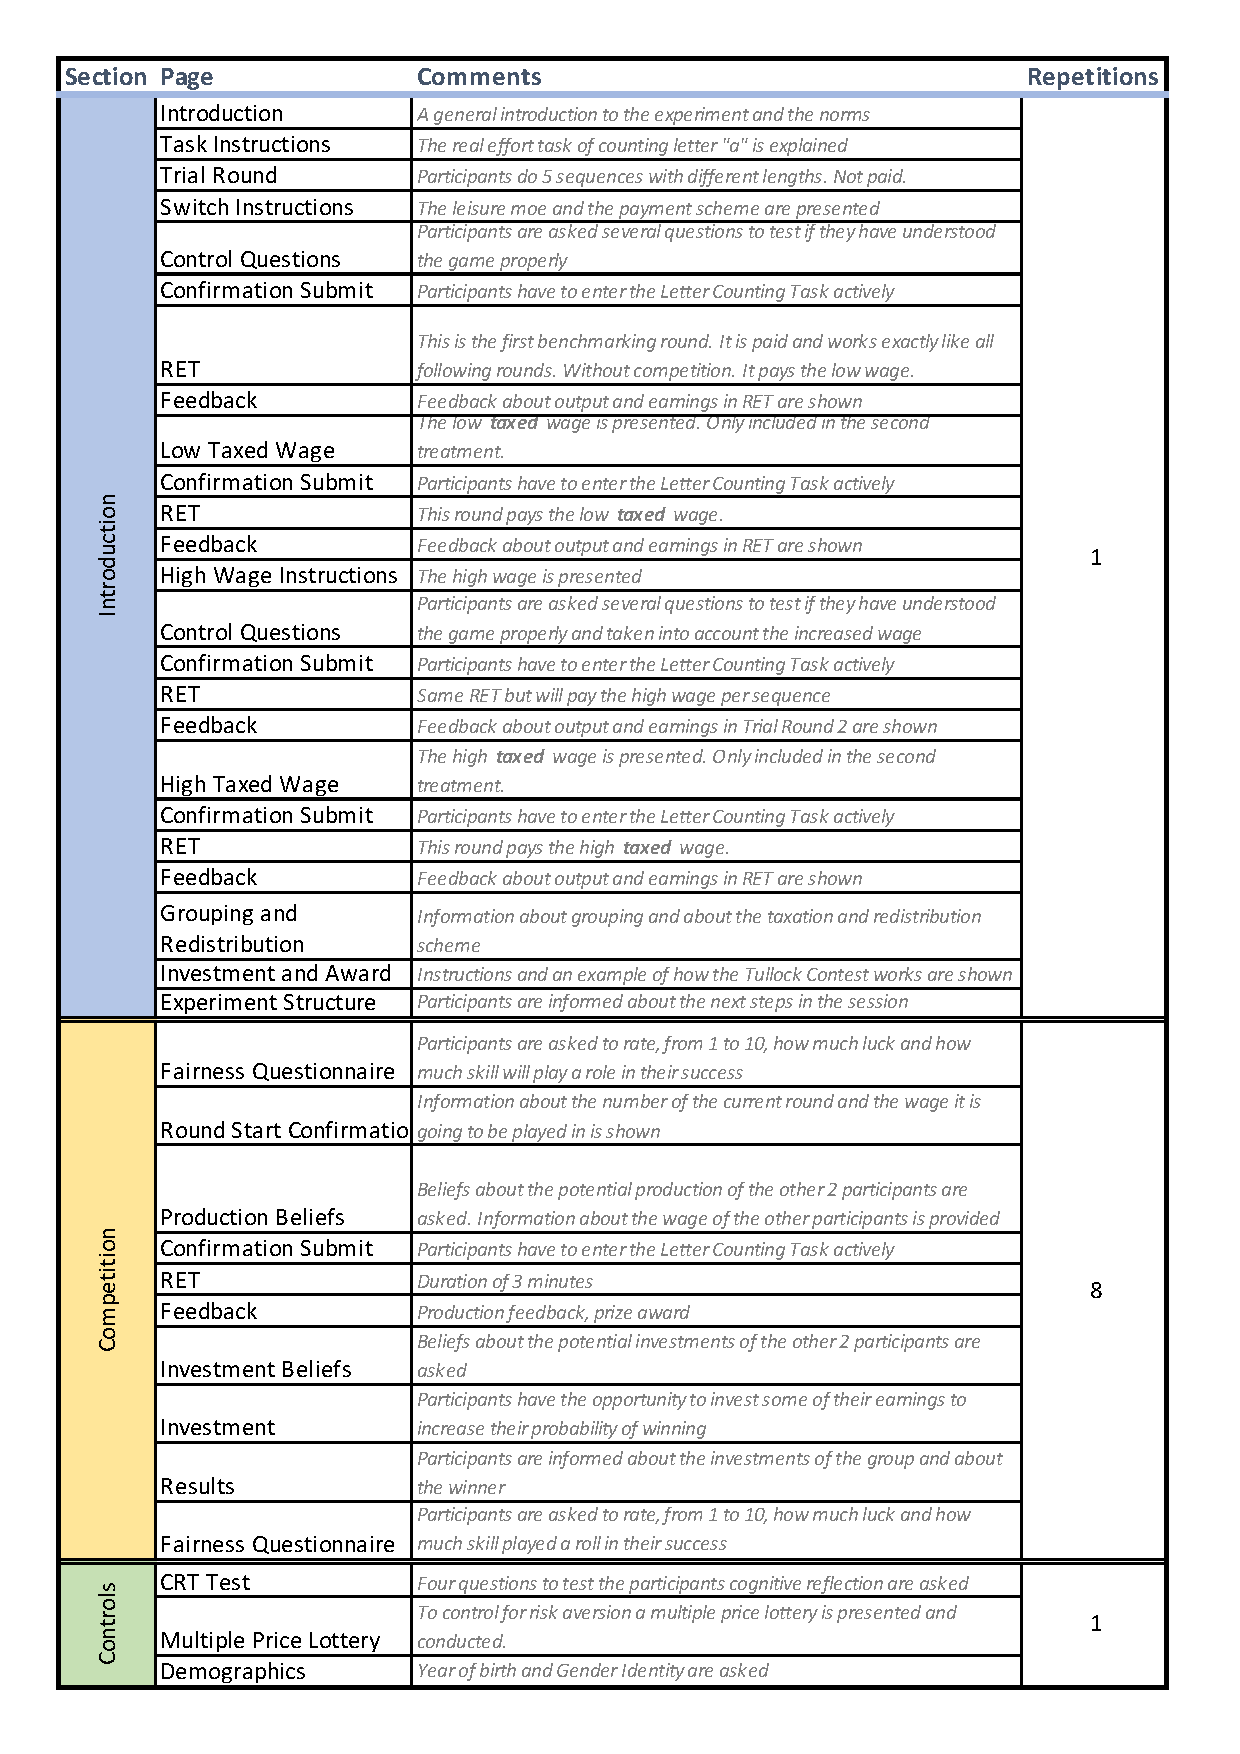
\includegraphics[width=\textwidth]{graphs/Experimental_Design.pdf}
        \caption{Detailed structure of the experiment}
        \label{tab:exp_design}
    \end{figure}

\chapter{Equations}

\section{Best Response for Winner in Round 2}

\begin{multline*}
y_i^* = \frac{1}{15}\cdot\\ \sqrt[3]{125 y_j^3 + 5400 y_j^2 + 18 \sqrt{330} \sqrt{125 y_j^4 + 5400 y_j^3 + 104490 y_j^2 + 373248 y_j} + 131220 y_j + 373248} - \\
\frac{-625 y_j^2 - 18000 y_j - 129600}{375 \sqrt[3]{125 y_j^3 + 5400 y_j^2 + 18 \sqrt{330} \sqrt{125 y_j^4 + 5400 y_j^3 + 104490 y_j^2 + 373248 y_j} + 131220 y_j + 373248}} - \\
2/15 (5 y_j - 36)
\end{multline*}

\section{Best Response for Loser in Round 2}

\begin{multline*}
y_j^* = \frac{1}{3} \sqrt[3]{a^3 + 30 a^2 + 3 \sqrt{33} \sqrt{2 a^4 + 60 a^3 + 897 a^2 + 2000 a} + 597 a + 1000}-\\
\frac{-a^2 - 20 a - 100}{3 \sqrt[3]{a^3 + 30 a^2 + 3 \sqrt{33} \sqrt{2 a^4 + 60 a^3 + 897 a^2 + 2000 a} + 597 a + 1000}} - \frac{2}{3} (a - 5)
\end{multline*}

\end{appendices}